\graphicspath{{images/stripes}}

\section{\thesection~Results}
\label{sec:results}
\citep{palkova1997}

\subsection{\thesubsection~Subsection}


% Make landscape and take a whole page.
% \end{multicols}
% \graphicspath{{images/comp_fit/}}
% \begin{Figure}
%   \centering
%   \includegraphics[width=\linewidth]{finals/P15_fit}
%   \captionof{figure}{(R5, C18) P15}
%   \label{fig:comp_fit_plate}
% \end{Figure}
% \begin{multicols}{2}


\end{multicols}
\graphicspath{{images/comp_fit/}}
\begin{Figure}
  \centering
  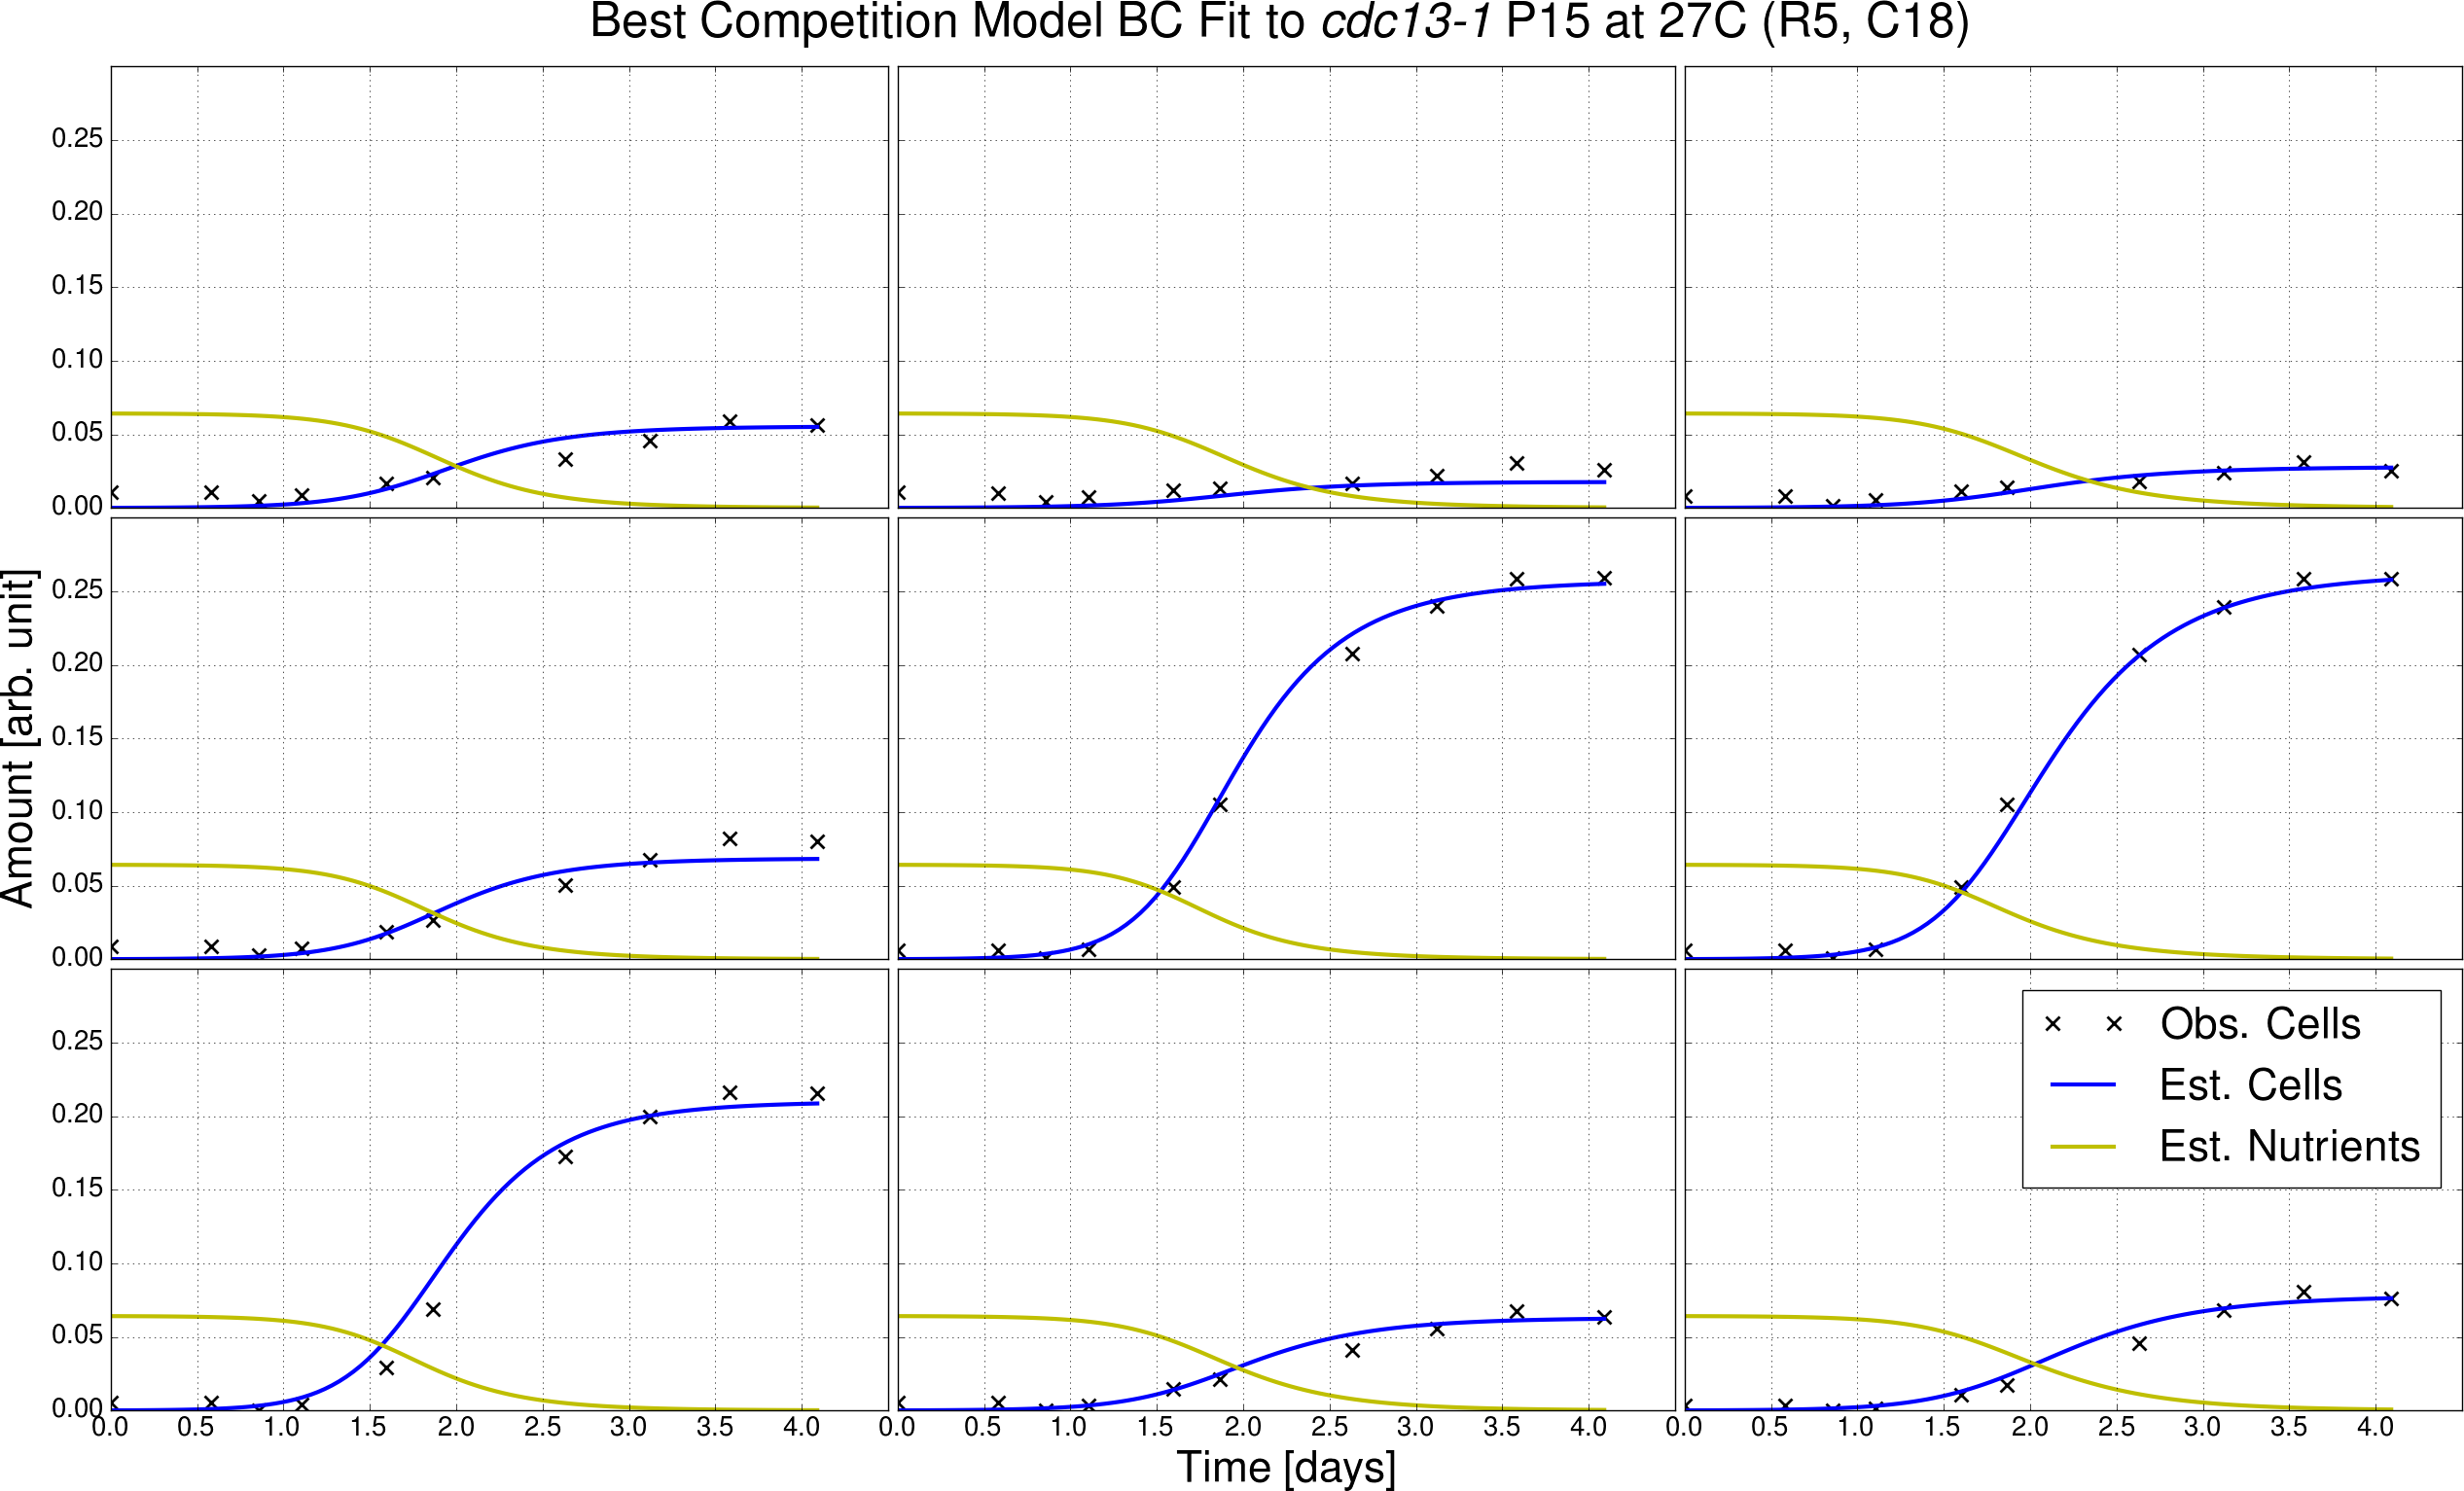
\includegraphics[width=\linewidth]{finals/P15_r5_c18_3x3}
  \captionof{figure}{(R5, C18) P15}
  \label{fig:comp_fit_zone}
\end{Figure}
\begin{multicols}{2}


\end{multicols}
\graphicspath{{images/stripes/}}
\begin{Figure}
  \centering
  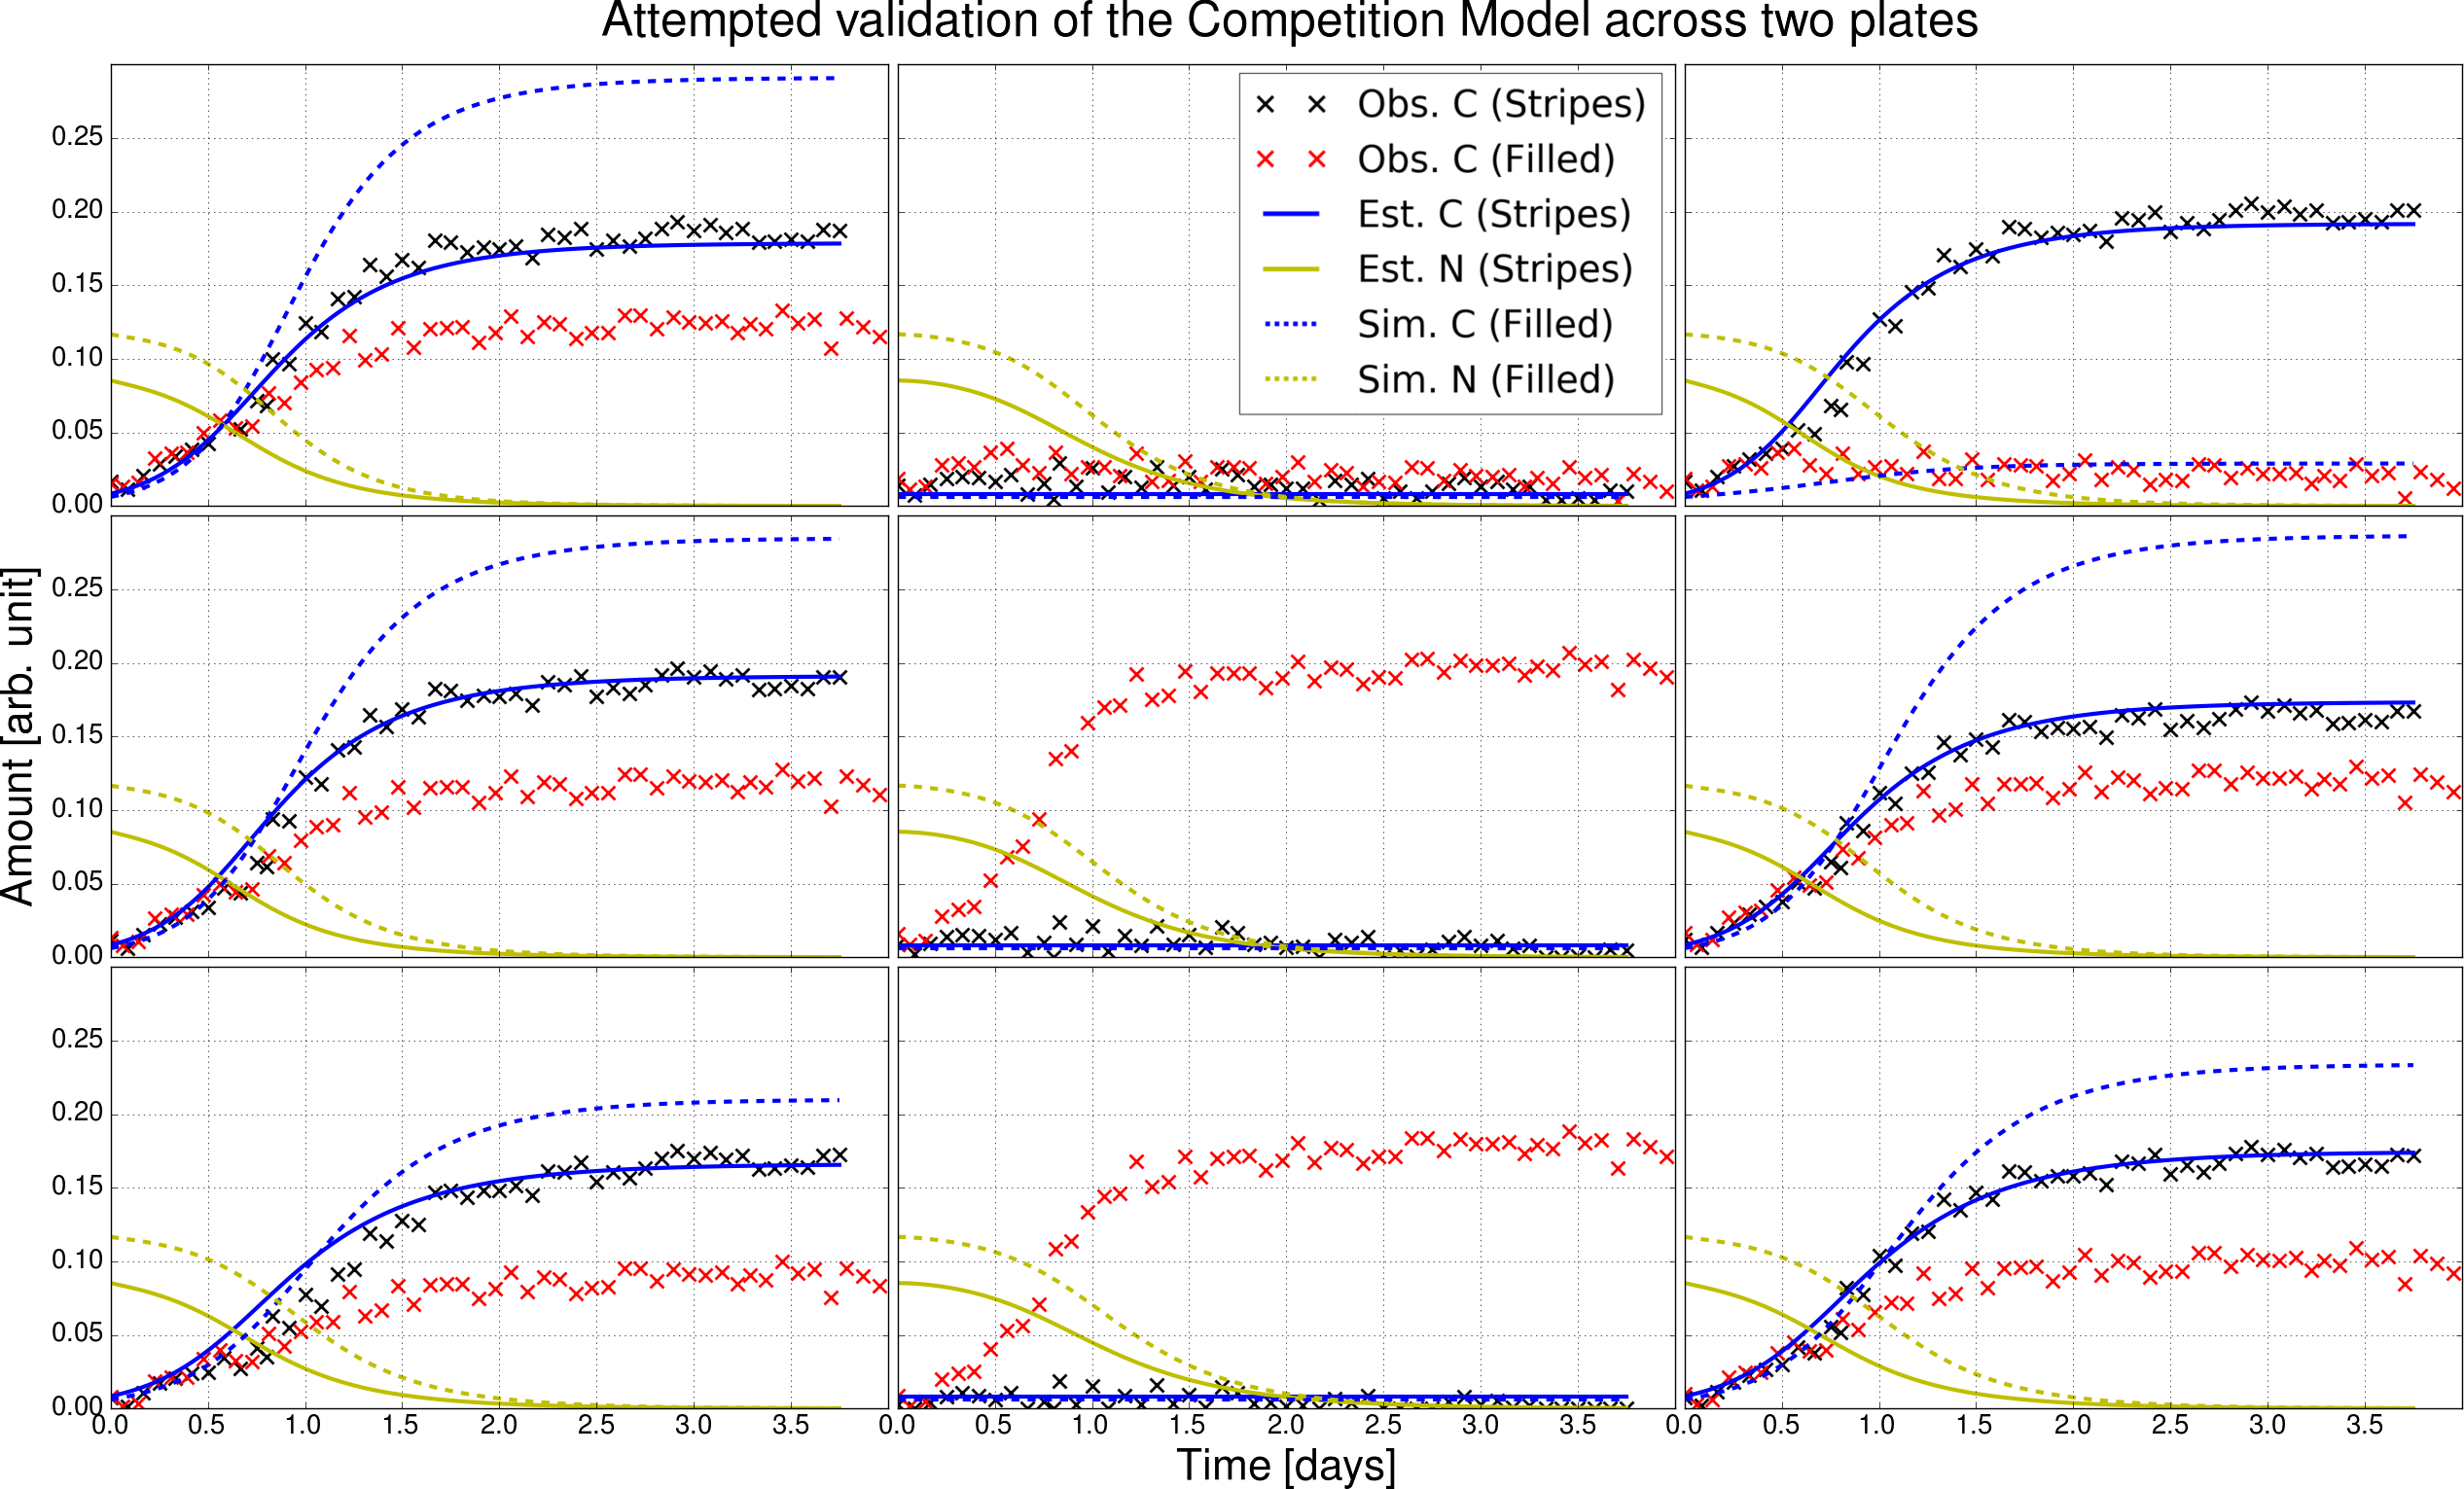
\includegraphics[width=\linewidth]{finals/validation_r9_c10}
  \captionof{figure}{(R9, C10) top-right possible pinning mistake. Bottom-left not close to any such mistake.}
  \label{fig:stripes_validation}
\end{Figure}
\begin{multicols}{2}

%%% Local Variables:
%%% mode: latex
%%% TeX-master: "report"
%%% End:
